\begin{frame}
    \titlepage
\end{frame}

{
\setbeamercolor{background canvas}{bg=blue!40!black,fg=blue!10!white}
\setbeamercolor{normal text}{bg=blue!40!black,fg=blue!10!white}
\setbeamercolor{itemize/enumerate body}{fg=white}
\setbeamercolor{itemize/enumerate subbody}{fg=white}
\setbeamercolor{titlelike}{bg=blue!40!black,fg=blue!10!white}
\begin{frame}<1|handout:1>[noframenumbering]{Changelog}
    \begin{itemize}
        \item Corrections made in this version not in first posting:
        \begin{itemize}
        \item 13 Feb 2017: slide 5: {\tt a\textbackslash*} instead of {\tt a\textbackslash}
        \end{itemize}
    \end{itemize}
\end{frame}
}

\begin{frame}{logistics: TRICKY}
    \begin{itemize}
    \item HW assignment out
    \item ``infecting'' an executable
    \end{itemize}
\end{frame}

\section{anti-virus techniques}

\begin{frame}<1>[label=antiVirusTech]{anti-virus techniques}
    \begin{itemize}
    \item last time: \myemph<2,5>{signature-based detection}
        \begin{itemize}
        \item regular expression-like matching
        \item snippets of virus(-like) code
        \end{itemize}
    \item \myemph<3>{heuristic detection}
        \begin{itemize}
        \item look for ``suspicious'' things
        \end{itemize}
    \item \myemph<4>{behavior-based detection}
        \begin{itemize}
        \item look for virus activity
        \end{itemize}
    \item not explicitly mentioned: \myemph<5>{producing signatures}
        \begin{itemize}
        \item manual? analysis
        \end{itemize}
    \item not explicitly mentioned: ``disinfection''
        \begin{itemize}
        \item manual? analysis
        \end{itemize}
    \end{itemize}
\end{frame}

\subsection{review: pattern matching}

\againframe<2>{antiVirusTech}

\begin{frame}[fragile,label=reCheat]{regular expression cheatsheet}
    \begin{itemize}
    \item {\tt a} --- matches {\tt a}
    \item {\tt a*} --- matches \textit{(empty string)}, {\tt a}, {\tt aa}, {\tt aaa}, \ldots
    \item {\tt a\textbackslash\*} --- matches the string {\tt a*}
    \item {\tt foo|bar} --- matches {\tt foo}, {\tt bar}
    \item {\tt [ab]} --- matches {\tt a}, {\tt b}
    \item \verb|[^ab]| --- matches any byte except a and b
    \item {\tt (foo|bar)*} ---
        \begin{itemize}
        \item \textit{(empty string)}, {\tt foo}, {\tt bar}, {\tt foobar}, {\tt barfoo}, \ldots
        \end{itemize}
    \item {\tt (.|\textbackslash{}n)*} --- matches anything whatsoever
    \end{itemize}
\end{frame}

\begin{frame}{recall: why regular expressions?}
    \begin{itemize}
    \item (essentially) one-pass, lookup table
    \item not the most flexible, but fast
    \vspace{.5cm}
    \item flex --- regular expressions + code for exceptions
    \end{itemize}
\end{frame}

\begin{frame}{recall: faster than regular expressions?}
    \begin{itemize}
    \item optimization 1: look for \myemph{fixed-length strings}
        \begin{itemize}
        \item sliding window + hashtable
        \item test with full pattern
        \end{itemize}
    \item optimization 2: \myemph{head/tail scanning}
        \begin{itemize}
        \item avoid reading whole files
        \end{itemize}
    \end{itemize}
\end{frame}

\begin{frame}[fragile,label=fixedScan]{scanning for fixed strings}
\begin{tikzpicture}
\tikzset{
    hideOnAdvance/.style={alt=<3>{opacity=0.2}{}},
    hideOnAdvance4/.style={alt={<3,4>{opacity=0.2}{}}},
    myline/.style={line width=0.7mm,-Latex,blue},
    hiString/.style={draw,blue,ultra thick,inner sep=.5mm},
}
\matrix[tight matrix,
    nodes={text width=.5cm,font=\tt\small}
] (string) {
    12 \& 34 \& 56 \& 78 \& 9A \& BC \& DE \& F0 \& 23 \& 45 \& 67 \& 89 \& AB \& CD \& EF \& 03 \& 45 \& 67 \& \ldots \\
};
\node[hideOnAdvance,hiString,fit=(string-1-2) (string-1-17)] (region) {};

\matrix[tight matrix,at={([yshift=-1cm,xshift=-.5cm]string.south east)},anchor=north east,
    nodes={text depth=.35mm},
    column 1/.style={nodes={font=\ttfamily\scriptsize,text width=6cm,
        alt=<4>{opacity=0.4}{}}},
    column 2/.style={nodes={font=\small\itshape,text width=2.2cm}},
    row 1/.style={nodes={font=\normalfont\small\bfseries}}] (patTable) {
    16-byte ``anchor'' \& malware \\
    204D616C6963696F7573205468696E6720 \& Virus A \\
    34567890ABCDEF023456789ABCDEFG0345 \& Virus B \\
    6120766972757320737472696E679090F2 \& Virus C \\
    \ldots                             \& \ldots \\
};
\draw[myline,hideOnAdvance] ([xshift=-4cm]region.south) |- (patTable-3-1.west);
\begin{visibleenv}<3->
\node[draw,minimum height=1cm,below=1.5cm of patTable,font=\itshape] (fulPat){
    (full pattern for Virus B)
};
\draw[myline,hideOnAdvance] (patTable-3-2.east) -- ++(.5cm,0cm) |- (fulPat.east);
\end{visibleenv}
\begin{visibleenv}<4>
\node[hiString,fit=(string-1-3) (string-1-18)] (regionB) {};
\end{visibleenv}
\begin{visibleenv}<5>
\node[draw,red,line width=.5mm,cross out,fit=(patTable-1-1) (patTable-4-1) (patTable.south west),
    inner sep=0mm] (theCross) {};
\begin{pgfonlayer}{fg}
\begin{visibleenv}<2->
\matrix[tight matrix,anchor=center,row sep=-.1mm,
    nodes={text depth=.35mm,fill=white,draw,thick},
    column 1/.style={nodes={font=\ttfamily\scriptsize,text width=3cm}},
    row 1/.style={nodes={font=\normalfont\small\bfseries}},
] (hashTable) at (theCross.center)
{
    4-byte hash \\
    FC923131 \\
    34598873 \\
    994254A3 \\
    \ldots \\
};
\draw[myline,red] ([xshift=-4cm]region.south) -- ++(0cm,-1cm) node[draw,fill=white] {hash function} |- (hashTable-3-1.west);
\end{visibleenv}
\end{pgfonlayer}
\end{visibleenv}
\end{tikzpicture}
\end{frame}

\begin{frame}{virus patterns}
    \begin{itemize}
    \item specific --- large snippet of code from virus
        \begin{itemize}
        \item false positives essentially impossible
        \end{itemize}
    \item general --- strategy (e.g. push + ret)
        \begin{itemize}
        \item false positives possible
        \item real applications might do this?
        \item might appear in application data?
        \end{itemize}
    \end{itemize}
\end{frame}

\subsection{new malware?}

\begin{frame}<1>[label=detectNew]{detecting new malware}
    \begin{itemize}
    \item goal: detect \myemph{unseen} malware
    \item some signatures might do this --- look for strategies
    \item also look for anomalies
        \begin{itemize}
        \item hope that real compilers/linkers/etc. don't do \ldots
        \end{itemize}
    \end{itemize}
\end{frame}

\subsection{heuristic: executable format messes}

\againframe<3>{antiVirusTech}

\begin{frame}{viruses and executable formats}
\begin{tikzpicture}
\tikzset{
    mybox/.style={draw,rectangle,minimum width=10cm,fill=white},
}
\node[mybox] (header) {
    \textbf{header}: machine type, file type, etc.
};
\node[mybox,below=0mm of header,align=center] (pHeader) {
    \textbf{program header}: ``\myemph{segments}'' to load \\
        (also, some other information) \\
    \only<2-3>{\myemph{\textbf{length edited by virus}}}
    \only<4-6>{\myemph{\textbf{new segment added by virus}}}
};
\node[mybox,below=0mm of pHeader,align=center] (seg1) {
    \textbf{segment 1 data}
};
\node[mybox,below=0mm of seg1,align=center] (seg2) {
    \textbf{segment 2 data} \\
    \only<2-3>{\myemph{\textbf{virus code + new entry point?}}}
};
\node[mybox,visible on=<4-6>,below=0mm of seg2,align=center] (seg3) {
    \myemph{\textbf{segment 3 data --- virus segment}}
};
\coordinate (annotate) at ([yshift=2.5cm]seg2.south);
\tikzset{
    annoBox/.style={draw=red,ultra thick,at=(annotate),align=center,fill=white},
}
\begin{visibleenv}<3,5>
    \node[annoBox] {heuristic 1: is entry point in last segment? \\ (last segment usually not code)};
\end{visibleenv}
\begin{visibleenv}<6>
    \node[annoBox] {heuristic 2: did virus mess up header? \\ (e.g. do sizes used by linker but not loader disagree)
                \\ section names disagree with usage?};
\end{visibleenv}
\end{tikzpicture}
\end{frame}

\begin{frame}{defeating entry point checking}
    \begin{itemize}
    \item \myemph<2>{insert jump in normal code section and\ldots}
        \begin{itemize}
        \item set as entry point; or
        \item assume it's reached `soon'
        \end{itemize}
    \end{itemize}
\begin{tikzpicture}[overlay,remember picture]
\coordinate (annotate) at ([yshift=-2cm]current page.center);
\tikzset{
    annoBox/.style={draw=red,ultra thick,align=center,fill=white,at=(annotate)},
}
    \begin{visibleenv}<2>
    \node[annoBox] {
        ``dynamic'' heuristic: run code in VM for a while, \\ see if switches sections
    };
    \end{visibleenv}
\end{tikzpicture}
\end{frame}

\subsection{heuristic: library call finding}

\begin{frame}{heuristics: library calls}
    \begin{itemize}
    \item dynamic linking --- functions called \myemph{by name}
    \item how do viruses add to dynamic linking tables?
        \begin{itemize}
        \item often don't! --- instead dynamically look-up functions
        \item if do --- could mess that up/lots of code
        \end{itemize}
    \end{itemize}

    \begin{tikzpicture}[overlay,remember picture]
    \coordinate (annotate) at ([yshift=-2cm]current page.center);
\tikzset{
    annoBox/.style={draw=red,ultra thick,fill=white,align=center,at=(annotate)},
}
    \node[annoBox] {
        heuristic: look for API function name strings \\ (outside linking info)
    };
    \end{tikzpicture}
\end{frame}

\begin{frame}{evading library call checking}
    \begin{itemize}
    \item modify dynamic linking tables
    \item reimplement library call manually
        \begin{itemize}
        \item Linux: usually easy
        \item Windows: system calls not well documented, change
        \end{itemize}
    \item \myemph<2>{hide names}
    \end{itemize}
\end{frame}

\begin{frame}{hiding library call names}
    \begin{itemize}
    \item common approach: store \myemph{hash of name}
    \item runtime: read library, scan list of functions for name
    \vspace{.5cm}
    \item bonus: makes analysis harder
    \end{itemize}
\end{frame}

\subsection{heuristic: behavior checking}

\againframe<4>{antiVirusTech}

\begin{frame}{behavior-based detection}
    \begin{itemize}
    \item things malware does that other programs don't?
    \vspace{.5cm}
    \item<2-> modify \myemph{system files}
    \item<2-> modifying \myemph{existing executables}
    \item<2-> open \myemph{network connections} to lots of random places 
    \item<2-> \ldots
    \vspace{.5cm}
    \item<3-> monitor all programs for weird behavior
    \item<3-> problem: false positives (e.g. installers)
    \end{itemize}
\end{frame}

\subsection{heuristic detection summary}

\begin{frame}{heuristic detection}
    \begin{itemize}
    \item virus ``shortcuts''
        \begin{itemize}
        \item generally: not producing executable via normal linker
        \item generally: trying to make analysis harder
        \item {\tt push} then {\tt ret} instead of {\tt jmp}
        \item entry point in ``wrong'' segment
        \item switching segments
        \item library calls without normal dynamic linker mechanisms
        \end{itemize}
    \item infection behavior
        \begin{itemize}
        \item modifying executables/system files
        \item weird network connections
        \end{itemize}
    \end{itemize}
\end{frame}

\subsection{heuristic case study}

\begin{frame}{example heuristics: DREBIN (1)}
    \begin{itemize}
    \item {\small from 2014 research paper on Android malware: Arp et al, ``DREBIN: Effective and Explainable Detection of Android Malware in Your Pocket''}
    \item features from applications (\myemph{without running}):
        \begin{itemize}
        \item hardware requirements
        \item requested permissions
        \item whether it runs in background, with pushed notifications, etc.
        \item what API calls it uses
        \item network addresses
        \end{itemize}
    \item detect \myemph{dynamic code generation} explicitly
    \item statistics (i.e. machine learning) to determine score
    \end{itemize}
\end{frame}

\begin{frame}{example heuristics: DREBIN (2)}
    \begin{itemize}
    \item advantage: Android uses Dalvik bytecode (Java-like)
        \begin{itemize}
        \item high-level ``machine code''
        \item much easier/more useful to analyze
        \end{itemize}
    \item accuracy?
        \begin{itemize}
        \item tested on 131k apps, $94$\% of malware, $1$\% false positives
        \item versus best commercial: $96$\%, $<0.3$\% false positives
            \begin{itemize}
            \item (probably has explicit patterns for many known malware samples)
            \end{itemize}
        \end{itemize}
    \item \ldots but
        \begin{itemize}
        \item statistics: training set needs to be typical of malware
        \item cat-and-mouse: what would attackers do in response?
        \end{itemize}
    \end{itemize}
\end{frame}

\section{antiantivirus}

\againframe<5>{antiVirusTech}

\begin{frame}{anti-anti-virus}
    \begin{itemize}
    \item defeating signatures:
    \vspace{.5cm}
    \item avoid things compilers/linkers never do
    \item make analysis harder
        \begin{itemize}
        \item takes longer to produce signatures
        \item takes longer to produce ``repair'' program
        \end{itemize}
    \item make changing viruses
        \begin{itemize}
        \item make any one signature less effective
        \end{itemize}
    \end{itemize}
\end{frame}

\begin{frame}{some terms}
    \begin{itemize}
    \item \myemph{armored} viruses
        \begin{itemize}
        \item viruses designed to make analysis harder
        \end{itemize}
    \item \myemph{metamorphic}/\myemph{polymorphic}/\myemph{oligomorphic} viruses
        \begin{itemize}
        \item viruses that change their code each time
        \item different terms --- different types of changes (later)
        \end{itemize}
    \end{itemize}
\end{frame}

\section{packers}

\subsection{intro: encrypted data}

\begin{frame}[fragile,label=encryptData]{encrypted(?) data}
\lstset{language=C,style=small}
\begin{lstlisting}
char obviousString[] =
    "Please open this 100%"
    " safe attachment";
char lessObviousString[] = 
    "oSZ^LZ\037POZQ\037KWVL\037\016\017"
    "\017\032\037L^YZ\037^KK^\\WRZQK";
for (int i = 0; i < sizeof(lessObviousString) - 1; ++i) {
    lessObviousString[i] =
        lessObviousString[i] ^ '?';
}
\end{lstlisting}
\end{frame}

\begin{frame}[fragile,label=recallHideAPI]{recall: hiding API calls}
\lstset{language=C,style=small}
\begin{lstlisting}
/* functions, functionsNames retrieved
   from library before */
/* 0xd7c9e758 = hash("GetFileAttributesA") */
unsigned hashOfString = 0xd7c9e758; 
for (int i = 0; i < num_functions; ++i) {
    unsigned functionHash = 0; 
    for (int j = 0; j < strlen(functionNames[i]); ++j) {
        functionHash = (functionHash * 7 +
                        functionNames[i][j]);
    }
    if (functionHash == hashOfString) {
        return functions[i];
    }
}
\end{lstlisting}
\end{frame}

\begin{frame}{encrypted data and signatures}
    \begin{itemize}
    \item doesn't really stop signatures
        \begin{itemize}
        \item ``encrypted'' string + decryption code is \myemph{more unique}
        \end{itemize}
    \item but makes \myemph{analyzing} virus a little harder
        \begin{itemize}
        \item how much harder?
        \item exercise: how would you decrypt strings?
        \end{itemize}
    \vspace{.5cm}
    \item<2-> can we do better?
    \end{itemize}
\end{frame}

\subsection{intro: encrypted code}

\begin{frame}[fragile,label=encrypted]{encrypted(?) viruses}
\lstset{language=C,style=small}
\begin{lstlisting}
char encrypted[] = "\x12\x45...";
char key[] = "...";
virusEntryPoint() {
    decrypt(encrypted, key);
    goto encrypted;
}
decrypt(char *buffer, char *key) {...}
\end{lstlisting}
\begin{itemize}
    \item choose a new key each time!
    \item not good encryption --- \myemph{key is there}
    \item sometimes mixed with \myemph{compression}
\end{itemize}
\end{frame}

\begin{frame}{encrypted viruses: no signature?}
    \begin{itemize}
    \item {\tt decrypt} is a pretty good signature
    \item still need to a way to disguise that code
    \vspace{.5cm}
    \item how about analysis? how does one analyze this?
    \end{itemize}
\end{frame}

\begin{frame}{not just anti-antivirus}
    \begin{itemize}
    \item ``encrypted'' body 
    \item just running objdump not enough\ldots
    \item instead --- run debugger, set \myemph{breakpoint} after ``decryption''
    \item \myemph{dump decrypted memory} afterwords
    \end{itemize}
\end{frame}

\begin{frame}{unneeded steps}
    \begin{itemize}
    \item understanding the ``encryption'' algorithm
        \begin{itemize}
        \item more complex encryption algorithm won't help
        \end{itemize}
    \item extracting the key and encrypted data
        \begin{itemize}
        \item making key less obvious won't help
        \end{itemize}
    \vspace{.5cm}
    \item<2-> needed to know \myemph{when encryption finished}
    \item<2-> needed debugger to work
    \item<3-> countermeasures?
        \begin{itemize}
        \item encrypt in strange order? multiple passes?
        \item anti-debugging (later)
        \end{itemize}
    \end{itemize}
\end{frame}

\subsection{example: Cascade}

\begin{frame}[fragile,label=cascade]{example: Cascade decrypter}
\lstset{
    style=small,
    language=myasm,
    moredelim={**[is][\btHL<2|handout:0>]{@hi2@}{@endhi@}},
    moredelim={**[is][\btHL<3|handout:0>]{@hi3@}{@endhi@}},
}
\begin{lstlisting}
    lea encrypted_code, %si
decrypt:
    mov $0x682, @hi3@%sp@endhi@ // length of body
    @hi2@xor %si, (%si)@endhi@
    @hi2@xor %sp, (%si)@endhi@
    inc %si
    dec @hi3@%sp@endhi@
    jnz decrypt
encrypted_code:
    ...
\end{lstlisting}
\imagecredit{Szor Listing 7.1}
\end{frame}

\subsection{decrypter variations}

\begin{frame}[fragile,label=decrypter]{decrypter}
    \begin{itemize}
    \item more variations:
        \begin{itemize}
        \item nested decrypters, different orders, etc.
        \end{itemize}
    \item still problem: \myemph{decrypter code is signature}
    \item \ldots but \myemph<2>{harder to distinguish\tikzmark{distinguish} different malware}
    \item often tries to \myemph<3>{frustrate debugging}\tikzmark{debugging} in other ways
        \begin{itemize}
        \item e.g. use stack pointer (not for the stack)
        \item (more on this later)
        \end{itemize}
    \end{itemize}

    \begin{tikzpicture}[overlay,remember picture]
        \begin{visibleenv}<2>
        \node[mycallout=distinguish,anchor=center] at ([yshift=-2cm]current page.center) {
            ``disinfection'' --- want to precisely identify malware
        };
        \end{visibleenv}

        \begin{visibleenv}<3>
        \node[mycallout=debugging,align=left,anchor=center] at ([yshift=-2cm]current page.center) {
            easiest way to defeat decrypter manually: \\
            run in debugger until code is decrypted
        };
        \end{visibleenv}
    \end{tikzpicture}
\end{frame}

\begin{frame}{legitimate ``packers''}
    \begin{itemize}
    \item some commercial software is packaged in this way
    \item \ldots including \myemph{antidebugging} stuff
    \vspace{.5cm}
    \item why? intended to be copy/reverse engineering protection
    \end{itemize}
\end{frame}

\section{metamorphic, etc.}

\begin{frame}<1>[label=playMouse,fragile]{playing mouse}
    \begin{itemize}
    \item signature-based techniques:
        \begin{itemize}
        \item \myemph<2>{scan for pattern of constant\tikzmark{constant} part of virus}
        \item \myemph<3>{scan for strings, approx. \tikzmark{fixed}16-bytes long}
        \item \myemph<4>{shortcut: scan \tikzmark{topBottom}top and bottom}
        \end{itemize}
    \item virus-writer hat: how can you defeat these?
        \begin{itemize}
        \item encrypting code? --- encrypter is pattern
        \end{itemize}
    \end{itemize}
    \begin{tikzpicture}[overlay,remember picture]
        %FIXME
        \coordinate (overlayLoc) at ([yshift=-2cm]current page.center);
        \tikzset{myover/.style={align=left,at=(overlayLoc),anchor=center}}
        \begin{visibleenv}<2>
        \node [mycallout=constant,myover] { change some trivial part of virus --- \\  e.g. add nops somewhere };
        \end{visibleenv}
        \begin{visibleenv}<3>
        \node [mycallout=fixed,myover] { insert nops everywhere; \\ split any big strings };
        \end{visibleenv}
        \begin{visibleenv}<4>
        \node [mycallout=topBottom,myover] { insert jump in middle \\ keep code out of end of file };
        \end{visibleenv}
    \end{tikzpicture}
\end{frame}

\subsection{oligomorphic viruses}

\againframe<2>{playMouse}

\begin{frame}{adding nops}
    \begin{itemize}
    \item instead of copying, copy but insert nops
    \item a little tricky --- only between instructions
    \item could have \myemph{hard-coded places} to insert
        \begin{itemize}
        \item likely easy to turn into signature
        \item or tricky to write
        \end{itemize}
    \item or can \myemph{parse instructions}
        \begin{itemize}
        \item x86 encoding isn't \textit{that bad}
        \item malware can use \myemph{limited subset}
        \end{itemize}
    \end{itemize}
\end{frame}

\begin{frame}{producing changing malware}
    \begin{itemize}
    \item not just {\tt nop}:
    \vspace{.5cm}
    \item switch between synonym instructions
    \item swap registers
    \item random instructions that manipulate `unused' register
    \item \ldots
    \end{itemize}
\end{frame}

\begin{frame}{oligomorphic viruses}
    \begin{itemize}
    \item use packing technique but
    \item make slight changes to decrypters
    \end{itemize}
\end{frame}

\subsubsection{case study: W95/Memorial}

\begin{frame}[fragile,label=W95Memorial]{example: W95/Memorial}
\lstset{
    style=small,
    language=myasm,
    moredelim={**[is][\btHL<2|handout:0>]{@hi2@}{@endhi@}},
    moredelim={**[is][\btHL<3|handout:0>]{@hi3@}{@endhi@}},
}
\begin{tabular}{ll}
\begin{lstlisting}
  @hi2@mov $0x405000, %ebp@endhi@
  @hi2@mov $0x550, %ecx@endhi@
  lea 0x2e(%ebp), %esi
  add 0x29(%ebp), %ecx
  mov 0x2d(%ebp), %al

decrypt:
  nop
  nop
  xor %al, (%esi)
  inc %esi
  nop
  inc %al
  @hi3@dec %ecx@endhi@
  @hi3@jnz decrypt@endhi@
  ...
\end{lstlisting}
&
\begin{lstlisting}
  @hi2@mov $0x550, %ecx@endhi@
  @hi2@mov $0x13bc000, %ebp@endhi@
  lea 0x2e(%ebp), %esi
  add 0x29(%ebp), %ecx
  mov 0x2d(%ebp), %al

decrypt:
  nop
  nop
  xor %al, (%esi)
  inc %esi
  nop
  inc %al
  @hi3@loop decrypt@endhi@
  ...
  ...
\end{lstlisting}
\end{tabular}
    \imagecredit{Szor, Listsings 7.3 and 7.4}
\begin{tikzpicture}[overlay,remember picture]
    \begin{visibleenv}<2>
    \node[anchor=center,draw=red,ultra thick,fill=white] at (current page.center) {
        change instruction order; location of decryption key/etc.
    };
    \end{visibleenv}
    \begin{visibleenv}<3>
    \node[anchor=center,draw=red,ultra thick,fill=white] at (current page.center) {
        variable choices of loop instructions
    };
    \end{visibleenv}
    \begin{visibleenv}<4>
    \node[anchor=center,draw=red,ultra thick,fill=white] at (current page.center) {
        Szor: ``96 different decryptor patterns''
    };
    \end{visibleenv}
\end{tikzpicture}
\end{frame}


\subsubsection{polymorphic /case study: 1260}

\begin{frame}{more advanced changes?}
    \begin{itemize}
    \item Szor calls W95/Memorial \myemph{oligomoprhic}
        \begin{itemize}
        \item ``encrypted'' code
        \item plus \myemph{small} changes to decrypter
        \end{itemize}
    \item What about doing more changes to decrypter?
        \begin{itemize}
        \item many, many variations
        \end{itemize}
    \item Szor calls doing this \myemph{polymorphic}
    \item polymorphic example: 1260
    \end{itemize}
\end{frame}

\begin{frame}[fragile,label=v1260]{example: 1260 (virus)}
\lstset{
    style=small,
    language=myasm,
    moredelim={**[is][\btHL<2-3|handout:0>]{@hi2@}{@endhi@}},
    moredelim={**[is][\btHL<4-5|handout:0>]{@hi3@}{@endhi@}},
}
% FIXME: adapt Listing 7.5
\begin{tabular}{ll}
\begin{lstlisting}
    @hi2@inc %si@endhi@
    mov @hi3@$0x0e9b@endhi@, %ax
    @hi2@clc@endhi@
    mov $0x12a, %di
    @hi2@nop@endhi@
    mov $0x571, %cx
decrypt:
    xor %cx, (%di)
    @hi2@sub %dx, %bx@endhi@
    @hi2@sub %cx, %bx@endhi@
    @hi2@sub %ax, %bx@endhi@
    @hi2@nop@endhi@
    @hi2@xor %cx, %dx@endhi@
    xor %ax, (%di)
    ...
\end{lstlisting}
&
\begin{lstlisting}
    mov @hi3@$0x0a43@endhi@, %ax
    @hi2@nop@endhi@
    mov $0x15a, %di
    @hi2@sub %dx, %bx@endhi@
    @hi2@sub %cx, %bx@endhi@
    mov $0x571, %cx
    @hi2@clc@endhi@
decrypt:
    xor %cx, (%di)
    @hi2@xor %cx, %dx@endhi@
    @hi2@sub %cx, %bx@endhi@
    @hi2@nop@endhi@
    @hi2@xor %cx, %bx@endhi@
    xor %ax, (%di)
    ...
\end{lstlisting}
\end{tabular}
\imagecredit{adapted from Szor, Listing 7.5}
\begin{tikzpicture}[overlay,remember picture]
    \begin{visibleenv}<3>
    \node[anchor=center,draw=red,ultra thick,fill=white] at (current page.center) {
        do-nothing instructions
    };
    \end{visibleenv}

    \begin{visibleenv}<5>
    \node[anchor=center,draw=red,ultra thick,fill=white] at (current page.center) {
        different decryption ``key''
    };
    \end{visibleenv}
\end{tikzpicture}
\end{frame}

\subsection{mutation engines generally}

\begin{frame}{lots of variation}
    \begin{itemize}
    \item essentially \myemph{limitless variations} of decrypter
        \begin{itemize}
        \item huge number of {\tt nop}-like sequences
        \item plus reordering non-{\tt nop} instructions
        \end{itemize}
    \item can't just make scanner that skips obvious {\tt nop}s
    \vspace{.5cm}
    \item<2-> could try to analyze more deeply for nops
        \begin{itemize}
        \item could identify when instruction's result is unused
        \end{itemize}
    \item<3-> but attacker can be more sophisticated:
        \begin{itemize}
        \item {\tt\fontsize{11}{12}\selectfont {\bfseries inc} \%ax; {\bfseries dec} \%ax}
        \item {\tt\fontsize{11}{12}\selectfont {\bfseries xor} \%ax, \%bx; {\bfseries xor} \%bx, \%ax; {\bfseries xor} \%ax, \%bx}
        \item \ldots
        \end{itemize}
    \end{itemize}
\end{frame}

\begin{frame}{interlude: anti-packer strategies}
\end{frame}

\section{heuristics for detecting packers}

\begin{frame}<1>[label=findingPackers]{finding packers}
    \begin{itemize}
    \item easiest way to decrypt self-decrypting code --- run it!
    \item solution: \myemph<1>{virtual machine} in antivirus software
    \vspace{.5cm}
    \item makes \myemph<2>{antivirtualization/emulation} more important
    \end{itemize}
\end{frame}

\begin{frame}{finding packers with VM}
    \begin{itemize}
    \item run program in VM for a while
        \begin{itemize}
        \item how long?
        \end{itemize}
    \item then scan memory for known patterns
    \item or detect jumping to written memory
    \end{itemize}
\end{frame}

\subsection{DEP}

\begin{frame}{stopping packers}
    \begin{itemize}
    \item it's \myemph<2>{unusual} to jump to code you wrote
    \item modern OSs: memory is executable or writable --- not both
    \end{itemize}
\end{frame}

\begin{frame}{diversion: DEP/{\tt W\textasciicircum X}}
    \begin{itemize}
    \item memory executable or writeable --- but not both
    \item exists for \myemph{exploits} (later in course), not packers
    \item requires hardware support to be fast (\myemph{early 2000s+})
    \item various names for this feature:
        \begin{itemize}
        \item Data Execution Prevention (DEP) (Windows)
        \item {\tt W\textasciicircum X} (``write XOR execute'')
        \item NX/XD/XN bit  (underlying hardware support)
            \begin{itemize}
            \item (No Execute/eXecute Disable/eXecute Never)
            \end{itemize}
        \end{itemize}
    \item \myemph{special system call} to switch modes
    \end{itemize}
\end{frame}

\begin{frame}{unusual, but\ldots}
    \begin{itemize}
    \item binary translation
        \begin{itemize}
        \item convert machine code to new machine code at runtime
        \end{itemize}
    \item Java virtual machine, JavaScript implementations
        \begin{itemize}
        \item ``just-in-time'' compilers
        \end{itemize}
    \item dynamic linkers
        \begin{itemize}
        \item load new code from a file --- same as writing code?
        \end{itemize}
    \item those packed commercial programs
    \vspace{.5cm}
    \item programs need to \myemph{explicitly} ask for write+exec
    \end{itemize}
\end{frame}

\section{antivirtualization}

\againframe<2>{findingPackers}

\begin{frame}<1>[label=antivirtIndex]{antivirtualization techniques}
    \begin{itemize}
    \item \myemph<2>{query virtual devices}
        \begin{itemize}
        \item<3> solution: mirror devices of some real machine
        \end{itemize}
    \item \myemph<4>{time operations that are slower in VM/emulation}
        \begin{itemize}
        \item<5> solution: virtual clock
        \end{itemize}
    \item \myemph<6>{use operations not supported by VM}
        \begin{itemize}
        \item<7> solution: support everything
        \end{itemize}
    \end{itemize}
\end{frame}

\againframe<2>{antivirtIndex}

\begin{frame}{virtual devices}
    \begin{itemize}
    \item VirtualBox device drivers?
    \item VMware-brand ethernet device?
    \item \ldots
    \end{itemize}
\end{frame}

\againframe<3-4>{antivirtIndex}

\begin{frame}{slower operations}
    \begin{itemize}
    \item not-``native'' VM:
        \begin{itemize}
        \item everything is really slow
        \end{itemize}
    \item otherwise --- trigger ``callbacks'' to VM implementation:
        \begin{itemize}
        \item system calls?
        \item allocating and accessing memory?
        \end{itemize}
    \item \ldots and hope it's reliably slow enough
    \end{itemize}
\end{frame}


\againframe<5-6>{antivirtIndex}

\begin{frame}{operations not supported}
    \begin{itemize}
    \item missing instructions kinds?
        \begin{itemize}
        \item FPU instructions
        \item MMX/SSE instructions
        \item undocumented (!) CPU instructions
        \end{itemize}
    \item not handling OS\tikzmark{OS} features?
        \begin{itemize}
        \item setting up special handlers for segfault
        \item multithreading
        \item system calls that make callbacks
        \item \ldots
        \end{itemize}
    \end{itemize}
    \begin{tikzpicture}[overlay,remember picture]
        \node[mycallout=OS,align=center,anchor=center] at ([yshift=-3cm]current page.center) {
            antivirus not running system VM to do decryption \\
            needs to emulate lots of the OS itself
        };
    \end{tikzpicture}
\end{frame}

\begin{frame}{attacking emulation patience}
    \begin{itemize}
    \item looking for unpacked virus in VM
    \item \ldots or other malicious activity
    \item when are you done looking?
    \vspace{.5cm}
    \item<2-> malware solution: \myemph<2>{take too long}
        \begin{itemize}
        \item not hard if emulator uses ``slow'' implementation
        \end{itemize}
    \item<3-> malware solution: \myemph<3>{don't infect consistently}
    \end{itemize}
\end{frame}

\begin{frame}[fragile,label=prob]{probability}
\lstset{language=C,style=smaller}
    \begin{tikzpicture}
    \node[draw,align=center] (malware) {
\begin{lstlisting}
if (randomNumber() == 4) {
    unpackAndRunEvilCode();
}
\end{lstlisting}
    };
    \node[draw,align=left,above right=1cm of malware] (avCase1) {
        antivirus emulator: \\
        \lstinline|randomNumber() == 3| \\
        \textbf{\color{green!60!black}looks clean!}
    }; 
    \node[draw,align=left,right=1cm of malware]  (avCase2) {
        real execution \#1: \\
        \lstinline|randomNumber() == 2| \\
        \textbf{\color{green!60!black}no infection!}
    }; 
    \node[draw,align=left,below right=1cm of malware] (avCase3) {
        real execution \#$N$: \\
        \lstinline|randomNumber() == 4| \\
        \textbf{\myemph{infect!}}
    }; 
    \draw[ultra thick,dashed,-Latex] (malware) -- (avCase1.west);
    \draw[ultra thick,dashed,-Latex] (malware) -- (avCase2.west);
    \draw[ultra thick,dashed,-Latex] (malware) -- (avCase3.west);
    \end{tikzpicture}
\end{frame}

\begin{frame}{on goats}
    \begin{itemize}
    \item analysis (and maybe detection) uses \textit{goat files}
    \item ``\myemph{sacrificial goat}'' to get changed by malware
    \item heuristics can avoid simple goat files, e.g.:
        \begin{itemize}
        \item don't infect small programs
        \item don't infect huge programs
        \item don't infect programs with huge amounts of {\tt nop}s
        \item \ldots
        \end{itemize}
    \end{itemize}
\end{frame}

\begin{frame}{goats as detection}
    \begin{itemize}
    \item tripwire for malware
    \item touching do-nothing {\tt .exe} --- very likely bad
    \end{itemize}
\end{frame}

\begin{frame}{goats as analysis}
    \begin{itemize}
    \item more important for analysis of \myemph{changing malware}
    \item want examples of \myemph{multiple versions}
    \item want it to be obvious where malware code added
        \begin{itemize}
        \item e.g. big cavities to fill in original
        \item e.g. obvious patterns in original code/data
        \end{itemize}
    \end{itemize}
\end{frame}

\section{metamorphic virsues}

\begin{frame}{changing bodies}
    \begin{itemize}
    \item ``decrypting'' a virus body gives body for ``signature''
        \begin{itemize}
        \item ``just'' need to run decrypter
        \end{itemize}
    \item how about avoiding static signatures entirely
    \item called \myemph{metamorphic}
        \begin{itemize}
        \item versus \myemph{polymorphic} --- only change ``decrypter''
        \end{itemize}
    \end{itemize}
\end{frame}

\begin{frame}[fragile,label=regSwap]{example: changing bodies}
\lstset{language=myasm,style=smaller}
\begin{tabular}{ll}
\begin{lstlisting}
pop %edx
mov $0x4h, %edi
mov %ebp, %esi
mov $0xC, %eax
add $0x88, %edx
mov (%edx), %ebx
mov %ebx, 0x1118(%esi,%eax,4)
\end{lstlisting}
&
\begin{lstlisting}
pop %eax
mov $0x4h, %ebx
mov %ebp, %esi
mov $0xC, %edi
add $0x88, %eax
mov (%eax), %esi
mov %esi, 0x1118(%esi,%eax,4)
\end{lstlisting}
\end{tabular}
\begin{itemize}
\item code above: after decryption
\item \myemph{every instruction} changes
\item still has good signatures
    \begin{itemize}
    \item with \myemph{alternatives} for each possible register selection
    \end{itemize}
\item but harder to write/slower to match
\end{itemize}
\end{frame}

\subsection{Evol example}

% FIXME
\begin{frame}<1>[fragile,label=caseEvol]{case study: Evol}
    \begin{itemize}
    \item via Lakhatia et al, ``Are metamorphic viruses really invincible?'', Virus Bulletin, Jan 2005.
    \item ``\myemph{mutation engine}''
        \begin{itemize}
        \item run as part of propagating the virus
        \end{itemize}
    \end{itemize}
    \begin{tikzpicture}
        \tikzset{
            every node/.style={font=\small,align=center},
            hiOn/.style={alt=<#1>{red,ultra thick}{}},
        }
        \path node[draw,hiOn=2] (disasm) {disassemble} -- ++(2.5cm,0) node (lens) {instr. \\ lengths} -- ++(2cm,0) node[draw,hiOn=3] (xform) {transform}
              -- ++(2cm,0) node[draw,hiOn=4] (reloc) {relocate};
        \node (origCode) at ([xshift=-2cm,yshift=1cm]disasm.north) {code};
        \node (finalCode) at ([xshift=2cm,yshift=-1cm]reloc.south) {code};
        \begin{scope}[thick,-Latex]
        \draw (origCode) |- (disasm);
        \draw (disasm) -- (lens);
        \draw (lens) -- (xform);
        \draw (xform) -- (reloc);
        \end{scope}
    \end{tikzpicture}
\end{frame}

\againframe<2>{caseEvol}

\begin{frame}{Evol instruction lengths}
    \begin{itemize}
    \item sounds really complicated?
    \item virus only handles instructions it has:
        \begin{itemize}
        \item about 61 opcodes, 32 of them identified by first four bits
            \begin{itemize}
            \item e.g. opcode {\tt 0x7\textit{x}} -- conditional jump
            \end{itemize}
        \end{itemize}
    \item no prefixes, no floating point
    \item only {\tt \%reg} or {\tt \$constant} or {\tt offset(\%reg)}
    \end{itemize}
\end{frame}

\againframe<3>{caseEvol}

\begin{frame}[fragile,label=evolXform]{Evol transformations}
\lstset{language=myasm,style=small}
    \begin{itemize}
    \item some stuff left alone
    \item static or random one of $N$ transformations
    \item example:
    \end{itemize}
\begin{tikzpicture}
\tikzset{
    every node/.style={font=\small,align=center}
}
\node[draw] (movebpEight) {
\begin{lstlisting}
mov %eax, 8(%ebp)
\end{lstlisting}
};

\node[draw,right=2cm of movebpEight] (movebpExpand) {
\begin{lstlisting}
push %ecx
mov %ebp, %ecx
add $0x12, %ecx
mov %eax, -0xa(%ecx)
pop %ecx
\end{lstlisting}
};
\node[anchor=north east] at ([yshift=-.25cm]movebpExpand.south east) {
    uses more stack space --- save temporary \\
    code gets bigger each time
};
\end{tikzpicture}
\imagecredit{Lakhotia et al., ``Are metamorphic viruses really invincible?'', Virus Bulletin, Jan 2005}
\end{frame}

\againframe<4>{caseEvol}

\begin{frame}{mutation with relocation}
    % FIXME: XXX
    \begin{itemize}
    \item table mapping old to new locations
        \begin{itemize}
        \item list of number of bytes generated by each transformation
        \end{itemize}
    \item list of locations references in original
        \begin{itemize}
        \item record relative offset in jump
        \item record absolute offset in original
        \end{itemize}
    \end{itemize}
\end{frame}

\begin{frame}[fragile,label=relocEx]{relocation example}
\lstset{language=myasm,style=small}
\begin{tikzpicture}
\node (code) {
\begin{lstlisting}
    mov ...
    mov ...
decrypt:
    xor %rax, (%rbx)
    inc %rbx
    dec %rcx
    jne decrypt
\end{lstlisting}
};
\matrix[tight matrix,nodes={font=\small},anchor=north west,
    nodes={font=\tt,text width=2cm,text depth=.1mm,minimum height=.4cm},
    row 1/.style={nodes={font=\small\bfseries,minimum height=1cm}},
    column 1/.style={text=blue!60!black,nodes={text width=1.75cm}},
    column 2/.style={text=green!60!black},
    column 3/.style={nodes={text width=1.5cm,font=\small\tt}},
] (lensTable) at ([xshift=1cm]code.north east) {
    orig. len \& new len \& instr \\
    5 \& 10 \& mov1 \\
    2 \& 3 \& mov2 \\
    2 \& 7 \& xor1 \\
    1 \& 1 \& inc1 \\
    1 \& 5 \& dec1 \\
    3 \& 3 \& jne1 \\
};
\matrix[tight matrix,nodes={font=\fontsize{9}{10}\selectfont,minimum height=1.2cm},anchor=north west,
    nodes={font=\tt,text width=4cm},
    row 1/.style={nodes={font=\small\bfseries,minimum height=1cm}},
    column 2/.style={text=blue!60!black},
    column 1/.style={text=green!60!black},
    column 3/.style={text=green!60!black},
] (relocTable) at ([yshift=-.5cm,xshift=-6.5cm]lensTable.south west) {
    address loc \& orig. target \& new target \\
    $10+3+7+1+5+1$ (jne1+1) \& xor1 ($5+2$)\& xor1 ($10+3$)\\ 
};
\end{tikzpicture}
\end{frame}

\begin{frame}{mutation engines}
    \begin{itemize}
    \item tools for writing polymorphic viruses
    \item best: \myemph{no} constant bytes, \myemph{no} ``no-op'' instructions
    \item tedious work to build state-machine-based detector
        \begin{itemize}
        \item ((almost) a regular expression to match it)
        \item apparently done manually
        \item automatable?
        \end{itemize}
    \item pattern: used until reliably detected
    \end{itemize}
\end{frame}


\begin{frame}[fragile,label=fancyMut]{fancier mutation}
    \begin{itemize}
    \item can do mutation on \myemph{generic machine code}
    \vspace{.5cm}
    \item ``just'' need full disassembler
    \item identify both \myemph{instruction lengths} and \myemph{addresses}
    \item hope machine code not written to rely on machien code sizes, etc.
    \item hope to identify \myemph{tables of function pointers}, etc.
    \end{itemize}
\end{frame}

\begin{frame}{fancier mutation}
    \begin{itemize}
    \item also an infection technique
        \begin{itemize}
        \item no ``cavity'' needed --- create one
        \end{itemize}
    \item obviously tricky to implement
        \begin{itemize}
        \item need to fix all executable headers
        \item what if you misparse assembly?
        \item what if you miss a function pointer?
        \end{itemize}
    \item example: Simile virus
    \end{itemize}
\end{frame}

\section{other antiantivirus}

% FIXME: move to index slide?
\begin{frame}<1>[label=moreantianti]{antiantivirus} 
    \begin{itemize}
    \item already covered:
        \begin{itemize}
        \item break disassemblers --- with packers
        \item break VMs/emulators
        \end{itemize}
    \item \myemph<2>{break debuggers}
        \begin{itemize}
        \item make analysis harder
        \end{itemize}
    \item \myemph<3>{break antivirus software itself}
        \begin{itemize}
        \item ``retrovirus''
        \end{itemize}
    \end{itemize}
\end{frame}


\subsection{anti-debugging}
\againframe<2>{moreantianti}

\begin{frame}<1>[label=debuggerThings]{diversion: debuggers}
    \begin{itemize}
    \item we'll care about two pieces of functionality:
    \vspace{.5cm}
    \item \myemph<2>{breakpoints}
        \begin{itemize}
        \item debugger gets control when certain code is reached
        \end{itemize}
    \item \myemph<3>{single-step}
        \begin{itemize}
        \item debugger gets control after a single instruction runs
        \end{itemize}
    \end{itemize}
\end{frame}

\againframe<2>{debuggerThings}

\begin{frame}[fragile,label=implBreak]{implementing breakpoints}
\lstset{language=myasm,style=small}
\begin{itemize}
    \item idea: change
\begin{lstlisting}
movq %rax, %rdx
addq %rbx, %rdx // BREAKPOINT HERE
subq 0(%rsp), %r8
...
\end{lstlisting}
into
\begin{lstlisting}
movq %rax, %rdx
jmp debugger_code 
subq 0(%rsp), %r8
...
\end{lstlisting}
    \item<2> problem: {\tt jmp} might be bigger than {\tt addq}?
\end{itemize}
\end{frame}

\begin{frame}[fragile,label=implBreak2]{int 3}
    \begin{itemize}
    \item x86 breakpoint instruction: {\tt \textbf{int} 3}
        \begin{itemize}
        \item Why 3? fourth entry in table of handlers
        \end{itemize}
    \item \myemph{one byte} instruction encoding: {\tt CC}
    \item debugger \myemph{modifies code to insert breakpoint}
        \begin{itemize}
        \item has copy of original somewhere
        \end{itemize}
    \item invokes handler setup by OS
        \begin{itemize}
        \item debugger can ask OS to be run by handler
        \item or changes pointer to handler directly on old OSes
        \end{itemize}
    \end{itemize}
\end{frame}

\begin{frame}{int 3 handler}
    \begin{itemize}
    \item kind of exception handler
        \begin{itemize}
        \item recall: exception handler = way for CPU to run OS code
        \end{itemize}
    \item x86 CPU saves registers, PC for debugger
    \item x86 CPU has easy to way to resume debugged code from handler
    \end{itemize}
\end{frame}

\begin{frame}[fragile,label=int3Check]{detecting int 3 directly (1)}
\lstset{language=myasm,style=small}
\begin{itemize}
    \item checksum running code
\end{itemize}
\begin{lstlisting}
mycode:
    ...
    movq $0, %rbx
    movq $mycode, %rax
loop:
    addq (%rax), %rbx
    addq $8, %rax
    cmpq $endcode, %rax
    jl loop
    cmpq %rbx, $EXPECTED_VALUE
    jne debugger_found
    ...
endcode:
\end{lstlisting}
\end{frame}

\begin{frame}[fragile,label=int3OSAPI]{detecting int 3 directly (2)}
\lstset{language=C,style=small}
\begin{itemize}
    \item query the ``handler'' for int 3
        \begin{itemize}
        \item old OSs only; today: cannot set directly
        \end{itemize}
    \item modern OSs: ask if there's a debugger attached
    \item \ldots or try to attach as debugger yourself
        \begin{itemize}
        \item doesn't work --- debugger present, probably
        \item does work --- broke any debugger?
        \end{itemize}
\end{itemize}
\begin{lstlisting}
 // Windows API function!
if (IsDebuggerPresent()) {
\end{lstlisting}
\end{frame}

\begin{frame}{modern debuggers}
    \begin{itemize}
    \item {\tt int 3} is the oldest x86 debugging mechanism
    \item modern x86: 4 ``breakpoint'' registers (\myemph{DR0--DR3})
        \begin{itemize}
        \item contain address of program instructions
        \item need more than 4? sorry
        \end{itemize}
    \item processor triggers exception when address reached
        \begin{itemize}
        \item 4 extra registers + comparators in CPU?
        \end{itemize}
    \item flag to invoke debugger if debugging registers used
        \begin{itemize}
        \item enables nested debugging
        \end{itemize}
    \end{itemize}
\end{frame}


\againframe<3>{debuggerThings}

\begin{frame}[fragile,label=implSingleStep]{implementing single-stepping (1)}
\lstset{language=myasm,style=small}
    \begin{itemize}
    \item set a breakpoint on the following instruction?
\begin{lstlisting}
movq %rax, %rdx
addq %rbx, %rdx // <-- STOPPED HERE
subq 0(%rsp), %r8 // <-- SINGLE STEP TO HERE
subq 8(%rsp), %r8
...
\end{lstlisting}
transformed to
\begin{lstlisting}
movq %rax, %rdx
addq %rbx, %rdx // <-- STOPPED HERE
int 3 // <-- SINGLE STEP TO HERE
subq 8(%rsp), %
...
\end{lstlisting}
then {\tt jmp} to {\tt addq}
    \item<2> but what about
\begin{lstlisting}
jmpq *0x1234(%rax,%rbx,8) // <-- STOPPED HERE
\end{lstlisting}
\end{itemize}
\end{frame}

\begin{frame}[fragile,label=implSingleStepB]{implementing single-stepping (2)}
\lstset{language=myasm,style=small}
    \begin{itemize}
    \item typically \myemph{hardware support} for single stepping
    \item x86:{\tt int 1} handler (second entry in table)
    \item x86: {\tt TF} flag: execute handler after every instruction
    \item \ldots except during handler (whew!)
    \end{itemize}
\end{frame}

\begin{frame}[fragile,label=defeatSingleStep]{Defeating single-stepping}
    \begin{itemize}
    \item try to install your own {\tt int 1} handler
        \begin{itemize}
        \item (if OS allows)
        \end{itemize}
    \item try to clear TF?
        \begin{itemize}
        \item would take effect on \myemph{following} instruction
        \item \ldots if debugger doesn't reset it
        \end{itemize}
    \end{itemize}
\end{frame}


\begin{frame}[fragile,label=unstealthyDebuggers]{unstealthy debuggers}
    \begin{itemize}
    \item is a debugger installed?
        \begin{itemize}
        \item unlikely on Windows, maybe ignore those machines
        \end{itemize}
    \item is a debugger process running (don't check if it's tracing you)
    \item \ldots
    \end{itemize}
\end{frame}

\begin{frame}{confusing debuggers}
    \begin{itemize}
    \item ``broken'' executable formats
        \begin{itemize}
        \item e.g., recall ELF: segments and sections
        \item corrupt sections --- program still works
        \item overlapping segments/sections --- program still works
        \end{itemize}
    \item use the stack pointer not for the stack
        \begin{itemize}
        \item stack trace?
        \end{itemize}
    \end{itemize}
\end{frame}

\subsection{retroviruses}

\againframe<3>{moreantianti}

\begin{frame}{attacking antivirus (1)}
    \begin{itemize}
    \item how does antivirus software scan new things?
        \begin{itemize}
        \item register handlers with OS/applications --- new files, etc.
        \end{itemize}
    \item how about registering your own?
    \end{itemize}
\end{frame}

\begin{frame}<1>[label=hookingList]{hooking}
    \begin{itemize}
    \item hooking --- getting a `hook' to run on (OS) operations
        \begin{itemize}
        \item e.g. creating new files
        \end{itemize}
    \item ideal mechanism: \myemph<2>{OS support}
    \item less ideal mechanism: \myemph<3>{change library loading}
        \begin{itemize}
        \item e.g. replace `open', `fopen', etc. in libraries
        \end{itemize}
    \item less ideal mechanism: \myemph<4>{replace OS exception} (system call) handlers
        \begin{itemize}
        \item very OS version dependent
        \end{itemize} 
    \end{itemize}
\end{frame}

\againframe<2>{hookingList}

\begin{frame}
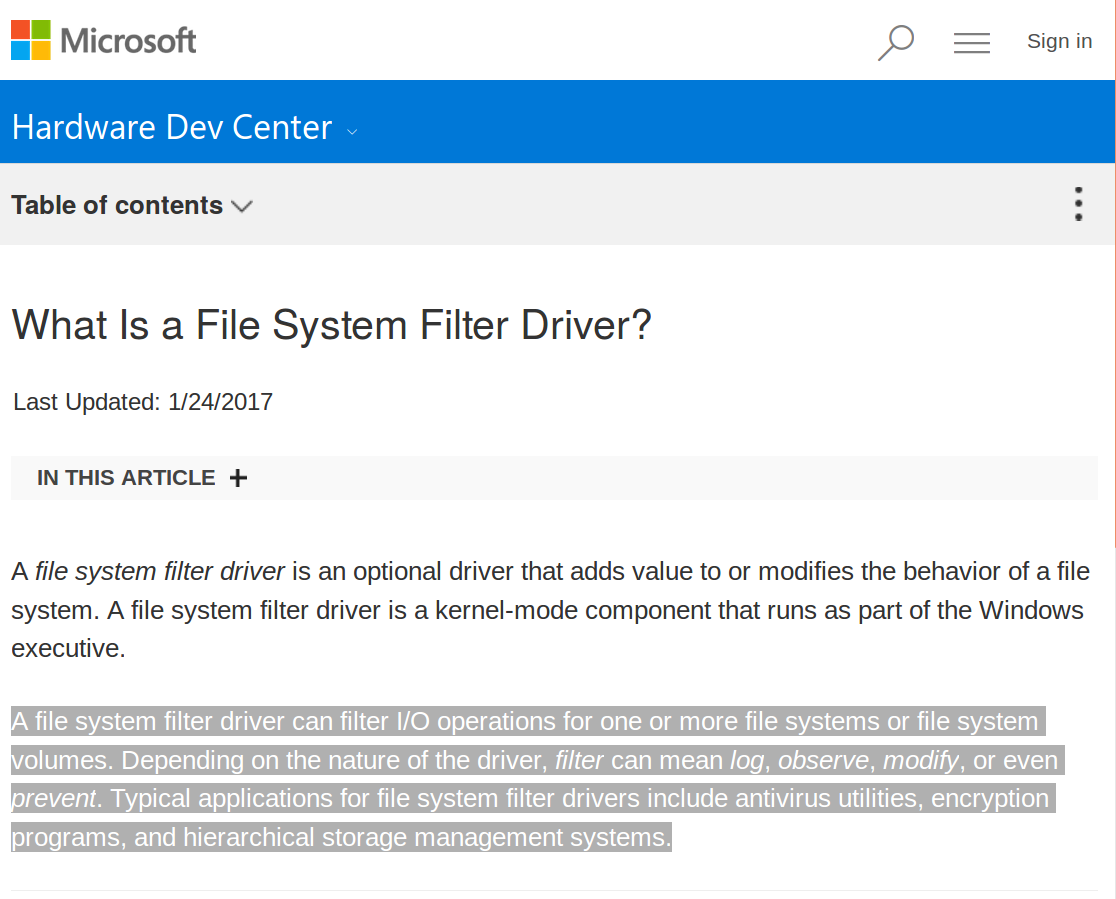
\includegraphics[height=0.9\textheight]{filter-driver}
\end{frame}

\againframe<3>{hookingList}

\begin{frame}{changing library loading}
\begin{itemize}
    \item e.g. install new library --- or edit loader, but \ldots
    \vspace{.5cm}
    \item not everything uses library functions
    \item what if your wrapper doesn't work exactly the same?
\end{itemize}
\end{frame}

\againframe<4>{hookingList}

\begin{frame}{attacking antivirus (2)}
    \begin{itemize}
    \item just directly modify it
        \begin{itemize}
        \item example: IDEA.6155 modifies database of scanned files
        \end{itemize}
    \item preserve checksums
        \begin{itemize}
        \item example: HybrisF preserved CRC32 checksums of infected files
        \item some AV software won't scan again
        \end{itemize}
    \end{itemize}
\end{frame}

\section{conclusion}

% FIXME: conclusion

\begin{frame}{armored viruses}
    \begin{itemize}
    \item ``encrypted'' viruses
        \begin{itemize}
        \item not strong encryption --- key is there!
        \end{itemize}
    \item self-changing viruses:
    \begin{tikzpicture}
    \begin{scope}[start chain=going right]
    \tikzset{
        every node/.style={font=\small,join,on chain},
        every join/.style={thick,Latex-Latex},
    }
    \node {encrypted};
    \node {oligiomorphic};
    \node {polymorphic};
    \node {metamorphic};
    \end{scope}
    \end{tikzpicture}
    \item breaking debuggers, antivirus
    \end{itemize}
\end{frame}

% FIXME: next time

\section{memory residence}

\begin{frame}{residence}
    \begin{itemize}
    \item our model of malware --- runs when triggered
    \item reality: sometimes keep on running
        \begin{itemize}
        \item evade active detection
        \item spread to new programs/files as created/run
        \end{itemize}
    \end{itemize}
\end{frame}

\section{recall: hooking}

% FIXME: bad hooking discussion

\subsection{DOS terminate-and-stay-resident}

\subsection{import table hooking}

\subsection{driver installation}

\section{stealth}

\subsection{semistealth --- directory breaking}

% FIXME: note nice infection marker like Vienna

\subsection{read stealth}


\section{Backup slides}
\begin{frame}{real signatures: ClamAV}
\begin{itemize}
\item ClamAV: open source email scanning software
\item signature types:
    \begin{itemize}
    \item hash of file
    \item hash of contents of segment of executable
        \begin{itemize}
        \item built-in executable, archive file parser
        \end{itemize}
    \item fixed string
    \item basic regular expressions
        \begin{itemize}
        \item wildcards, character classes, alternatives
        \end{itemize}
    \item more complete regular expressions
        \begin{itemize}
        \item including features that need more than state machines
        \end{itemize}
    \item meta-signatures: match if other signatures match
    \item icon image fuzzy-matching
    \end{itemize}
\end{itemize}
\end{frame}
